\documentclass[17pt]{beamer} %Makes presentation
%\documentclass[handout]{beamer} %Makes Handouts
\usetheme{Singapore} %Gray with fade at top
\useoutertheme[subsection=false]{miniframes} %Supppress subsection in header
\useinnertheme{rectangles} %Itemize/Enumerate boxes
\usecolortheme{seagull} %Color theme
\usecolortheme{rose} %Inner color theme

\definecolor{light-gray}{gray}{0.75}
\definecolor{dark-gray}{gray}{0.55}
\setbeamercolor{item}{fg=light-gray}
\setbeamercolor{enumerate item}{fg=dark-gray}

\setbeamertemplate{navigation symbols}{}
%\setbeamertemplate{mini frames}[default]
%\setbeamercovered{dynamics}
\setbeamerfont*{title}{size=\Large,series=\bfseries}
\setbeamerfont{footnote}{size=\tiny}

%\setbeameroption{notes on second screen} %Dual-Screen Notes
%\setbeameroption{show only notes} %Notes Output

\setbeamertemplate{frametitle}{\vspace{.5em}\bfseries\insertframetitle}
\newcommand{\heading}[1]{\noindent \textbf{#1}\\ \vspace{1em}}

\usepackage{bbding,color,multirow,times,ccaption,tabularx,graphicx,verbatim,booktabs}
\usepackage{colortbl} %Table overlays
\usepackage[english]{babel}
%\usepackage[latin1]{inputenc}
%\usepackage[T1]{fontenc}
\usepackage{lmodern}

%\author[]{Thomas J. Leeper}
\institute[]{
  \inst{}%
  Department of Government\\London School of Economics and Political Science
}

\usepackage{tikz}
\usetikzlibrary{shapes,arrows,positioning}

\title{Theory Development and Hypothesis Generation}

% How do we create social science theories based on past evidence and novel observation? What roles do induction and deduction play in contemporary political science?

\date[]{}

\begin{document}

\frame{\titlepage}

\frame{\tableofcontents}


% Add a thing about annotated bibliographies



\section{Theory}
\frame{\tableofcontents[currentsection]}



\frame{
\frametitle{Scientific method}

\begin{enumerate}
\item Research question(s)
\item Clarify the core concepts
\item \textbf{Develop theory}
\item Derive specific, testable hypotheses
\item Plan data collection
\item Gather data/evidence
\item Analyze data
\item Draw inferences
\end{enumerate}

}

\frame{
\frametitle{{\large Key Points from MT}}

\begin{enumerate}\itemsep1em
\item Theory is about concepts
\item Analysis is about measured variables
\item So our task as scientists is to:
	\begin{itemize}
	\item Find observable implications of theory
	\item Draw theoretical implications from measures
	\end{itemize}
\end{enumerate}
}


\frame{

\begin{center}
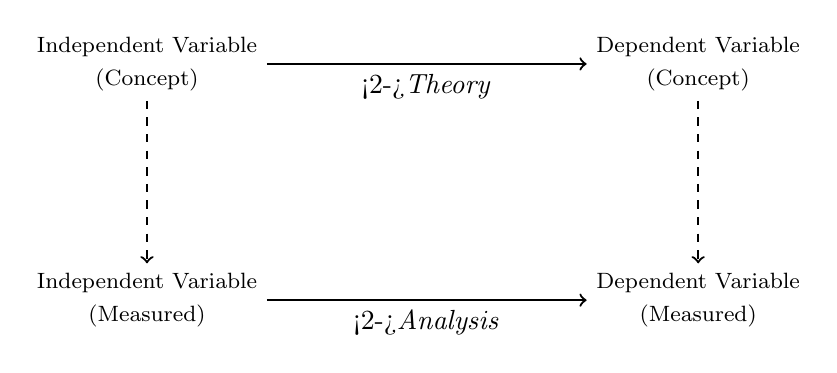
\begin{tikzpicture}
\node [align=center] (ivm) at (0,0) {\footnotesize Independent Variable\\\footnotesize (Measured)};
\node [align=center] (dvm) at (7,0) {\footnotesize Dependent Variable\\\footnotesize (Measured)};

\node [align=center] (ivc) at (0,3) {\footnotesize Independent Variable\\\footnotesize (Concept)};
\node [align=center] (dvc) at (7,3) {\footnotesize Dependent Variable\\\footnotesize (Concept)};

\node (analysis) at (3.5, 0) {};
\node (theory) at (3.5, 3) {};

\draw [->, thick] (ivm) -- (dvm) node[midway, below] (analysis) {{\only<2->{\textit{Analysis}}}};
\draw [->, thick] (ivc) -- (dvc) node[midway, below] (theory) {{\only<2->{\textit{Theory}}}};
\draw [->, dashed, thick] (ivc) -- (ivm);
\draw [->, dashed, thick] (dvc) -- (dvm);
\end{tikzpicture}
\end{center}


}


\frame{}

\frame{

\frametitle{{\large What is a theory?}}

\begin{itemize}\itemsep1em
\item Kellstedt and Whitten's definition:\footnote{Kellstedt and Whitten, p.3}\\
A tentative conjecture about the causes of some phenomenon of interest
\item<2-> Another way of saying this:\\
An \alert<3>{argument} that attempts to \alert<3>{explain} how concepts are causally related
\end{itemize}

}

% theories are arguments and they are (potential) explanations
% concepts may also be hierarchical - some are grand, macro theories; others are small micro theories and it may be that the micro theories build on macro theories

% there are also descriptive theories, e.g., typologies (Presidential character, welfare states, )



\frame{

\frametitle{Generating Theory I}

\begin{itemize}\itemsep0.5em
\item One way to theorize is to reason \textit{inductively} % bottom-up appraoch

\item Induction works by drawing generalities from specific observations

\item Sometimes called ``bottom-up'' theorizing
\end{itemize}

}

% activity to practice inductive reasoning
%% why do people vote or why do people not vote?

%% perhaps gender differences in female legislative representation?


\frame{

\frametitle{Generating Theory II}

\begin{itemize}\itemsep0.5em
\item An alternative way of developing theory is through \textit{deduction} 

\item Deduction begins from general, assumed principles/axioms to reach more specific observable realities % top-down approach

\item<2-> Common example: Rational choice theory

\end{itemize}

}

% the first calculus of voting (Arrow; Downs) was purely deductive


\frame<1>[label=theory1]{

\frametitle{Generating Theory III}

\begin{itemize}\itemsep0.5em
\item ``The Calculus of Voting'' is a \textit{rational choice} theory
	\begin{itemize}
	\item Assumes utility maximization is the driver of all behaviour
	\item Understanding phenomena is a matter of figuring out utility structures, especially those created by institutions
	\end{itemize}
\item<2-> Not the only broad theoretical paradigm
\end{itemize}
}


\frame{

\frametitle{The Calculus of Voting}

\small

Theory: Voting is explained by \only<1>{3}\only<2>{4} factors\\

\begin{columns}
  \begin{column}{0.45\textwidth}
    \begin{itemize}
	\item Costs of voting
	\item Benefits from preferred alternative winning
	\item Probability of impacting result
	\item<2-> Benefits from voting \textit{per se}
    \end{itemize}
  \end{column}
  
  \begin{column}{0.55\textwidth}
  \tikzstyle{block} = [rectangle, draw, text width=2cm, text centered, rounded corners, minimum height=1em, node distance=9cm]
  \begin{tikzpicture}[scale=0.3]
  \draw<1-> [block] node at (0,0) (voting) {{\small Pr(Voting)}};
  \draw<1-> [block, above left of=voting] node (costs) {{\small Costs}};
  \draw<1-> [block, left of=voting] node (ben) {{\small Benefits}};
  \draw<1-> [block, below left of=voting] node (p) {{\small Pr(Impact)}};
  \draw<2-> [block, below of=voting] node (d) {{\small ``D term''}};
  \draw<1-> [->, very thick] (costs) -- (voting);
  \draw<1-> [->, very thick] (ben) -- (voting);
  \draw<1-> [->, very thick] (p) -- (voting);
  \draw<2-> [->, very thick] (d) -- (voting);
  \end{tikzpicture}
  
  \end{column}
\end{columns}

}


% other examples of this:
% logic of collecive action; selective incentives; Mancur Olson
% common pool resource problems; communication and sanctions; Elinor Ostrom

% an example: calculus of voting



\frame{

\frametitle{Aside: Assumptions}

\begin{center}
If a theory require assumptions, is that theory credible?
\end{center}

}

% there are debates about whether it is okay to make assumptions that we do not test (see, e.g., Kahneman and Tversky)
% there are also debates about whether theories are useful independent of whether they explain the world as it is (see, e.g., Clark and Primo)

\againframe{theory1}



\frame{

\frametitle{The Michigan Model}

\small

Theory: Vote choice is explained by long-standing partisan identification, which is in turn shaped by early socialization.

\vspace{2em}

\tikzstyle{block} = [draw, text width=2.5cm, minimum height=1em, node distance=8cm]
\begin{tikzpicture}[scale=0.75]
\draw [block] node at (0,0) (voting) {{\small Vote Choice}};
\draw [block] node at (-5,0) (pid) {{\small Party\\ Identification}};
\draw [block] node at (-10,1.5) (p) {{\small Parental\\ Party ID}};
\draw [block] node at (-10,-1.5) (e) {{\small Early Adult\\ Experiences}};
\draw [->, very thick] (p) -- (pid);
\draw [->, very thick] (e) -- (pid);
\draw [->, very thick] (pid) -- (voting);
\end{tikzpicture}
}




\frame{

\frametitle{Induction vs. Deduction?}

\begin{itemize}\itemsep0.5em
\item Induction and deduction are both integral to science

% example: the calculus of voting; modified theory based on new evidence

\item Theory testing and theory building both require observation
\end{itemize}

}

% the second calculus of voting (Riker and Ordeshook) was partly inductive

% theory development is separate from theory testing
% but the two are interrelated



% induction (bottom up) vs. deduction (top down; from theory to observation)
% generally, in political science, we are interested in building theories from earlier more acceptable theoretical premises
% if we believe the world operates in some way, we can draw more specific conjectures about features of the world
% and then test those conjectures using evidence

% yet, the result is that when we collect evidence, sometimes we falsify (or fail to find evidence in support of) our theories
% the results is that we must either amend our premises, amend our argument, or set scope conditions on theory

% these theories then become useful because by drawing generalities about the world, we are able to understand particular events
% when those particular events then deviate from expectations, it invites renewed theorizing, amendment of argument, or the implication of scope conditions

% so science is both deductive and inductive, though the way we talk about science is typically deductive


% in the end, however, our goal is to "explain" the world...that has to start from a mix of assumption-based theory, theory development expanding on previously validated theory, and novel data collection


\frame{

\frametitle{Theory Generation in Practice}

As you theorize an explanation for some phenomenon, you will draw on:

\begin{itemize}\itemsep1em
\item General principles
\item Extant theory
% application; generalization; moderation; scope conditions; proposing mechanisms for extant relationships
\item Specific evidence
% don't use the evidence we will eventually test our theory on
\end{itemize}

}


\frame{

\frametitle{{\large What makes for a good theory?}}

\begin{itemize}
\item Truth
\item Falsifiability
\item Relevance
\item Coherence
\item Generality
\item Parsimony
\end{itemize}

}

\frame{

\frametitle{Generality \& Parsimony}

Think for 90 seconds about each of these principles:

\small 

\begin{itemize}\itemsep1em
\item Generality: Theories that can explain more are preferred over theories that can explain less
\item Parsimony: Simple theories are preferred over complex theories
\end{itemize}

\normalsize

Are these principles defensible?\\ Are they any good?

}


\section{Generating Hypotheses}
\frame{\tableofcontents[currentsection]}


\frame{

\frametitle{Hypotheses}

\begin{itemize}\itemsep0.5em
\item<2-> Definition: a theory-based statement about a relationship that we expect to observe.\footnote{Kellstedt and Whitten (p.4)}

\item<3-> Features
	\begin{itemize}
	\item Derived from theory
	\item Specific
	\item Empirical/observable
	\end{itemize}
\end{itemize}

}

% we cannot test theory; we can only test observable implications of theory
% hypotheses are statements about observable implications
% finding support for a hypothesis is evidence in support of a theory
% finding lack of support for a hypothesis is evidence against a theory



\frame{

\frametitle{How do we generate hypotheses?}

\begin{itemize}\itemsep0.5em
\item Think about \textit{observable implications}
\item What would evidence consistent with this theory be?
\item What would evidence inconsistent with this theory be?
	\begin{itemize}
	\item<2-> This is \textit{falsifiability}
	\end{itemize}
\end{itemize}

}

% falsifiability
	% typically talked about in descriptive terms (all swans are white)
	% can be harder to think of non-falsifiable causal arguments
		% theories without observable implications (homeopathy; remote viewing)
		% ethics are non-falsifiable without a predetermined set of rules governing what is and is not ethical

% Examples from Rosenbaum


\frame{

\frametitle{Example: Broad Street Cholera}

\begin{itemize}\itemsep0.5em
\item 1854 outbreak of cholera in London
	\begin{itemize}
	\item Around Broad Street (Soho)
	\item 616 eventual deaths
	\end{itemize}
\item<2-> What causes transmission of cholera?
\item<3-> Dominant theory at time: ``miasma''
\item<4-> Hypotheses:
	\begin{itemize}
	\item Clean up garbage $\rightarrow\hspace{1em} \downarrow$ cholera
	\item Open windows $\rightarrow \hspace{1em} \downarrow$ cholera
	\end{itemize}
\end{itemize}

}

% miasmatic theory of disease (``bad air''); dominant since the bubonic plague


\frame{

\begin{center}
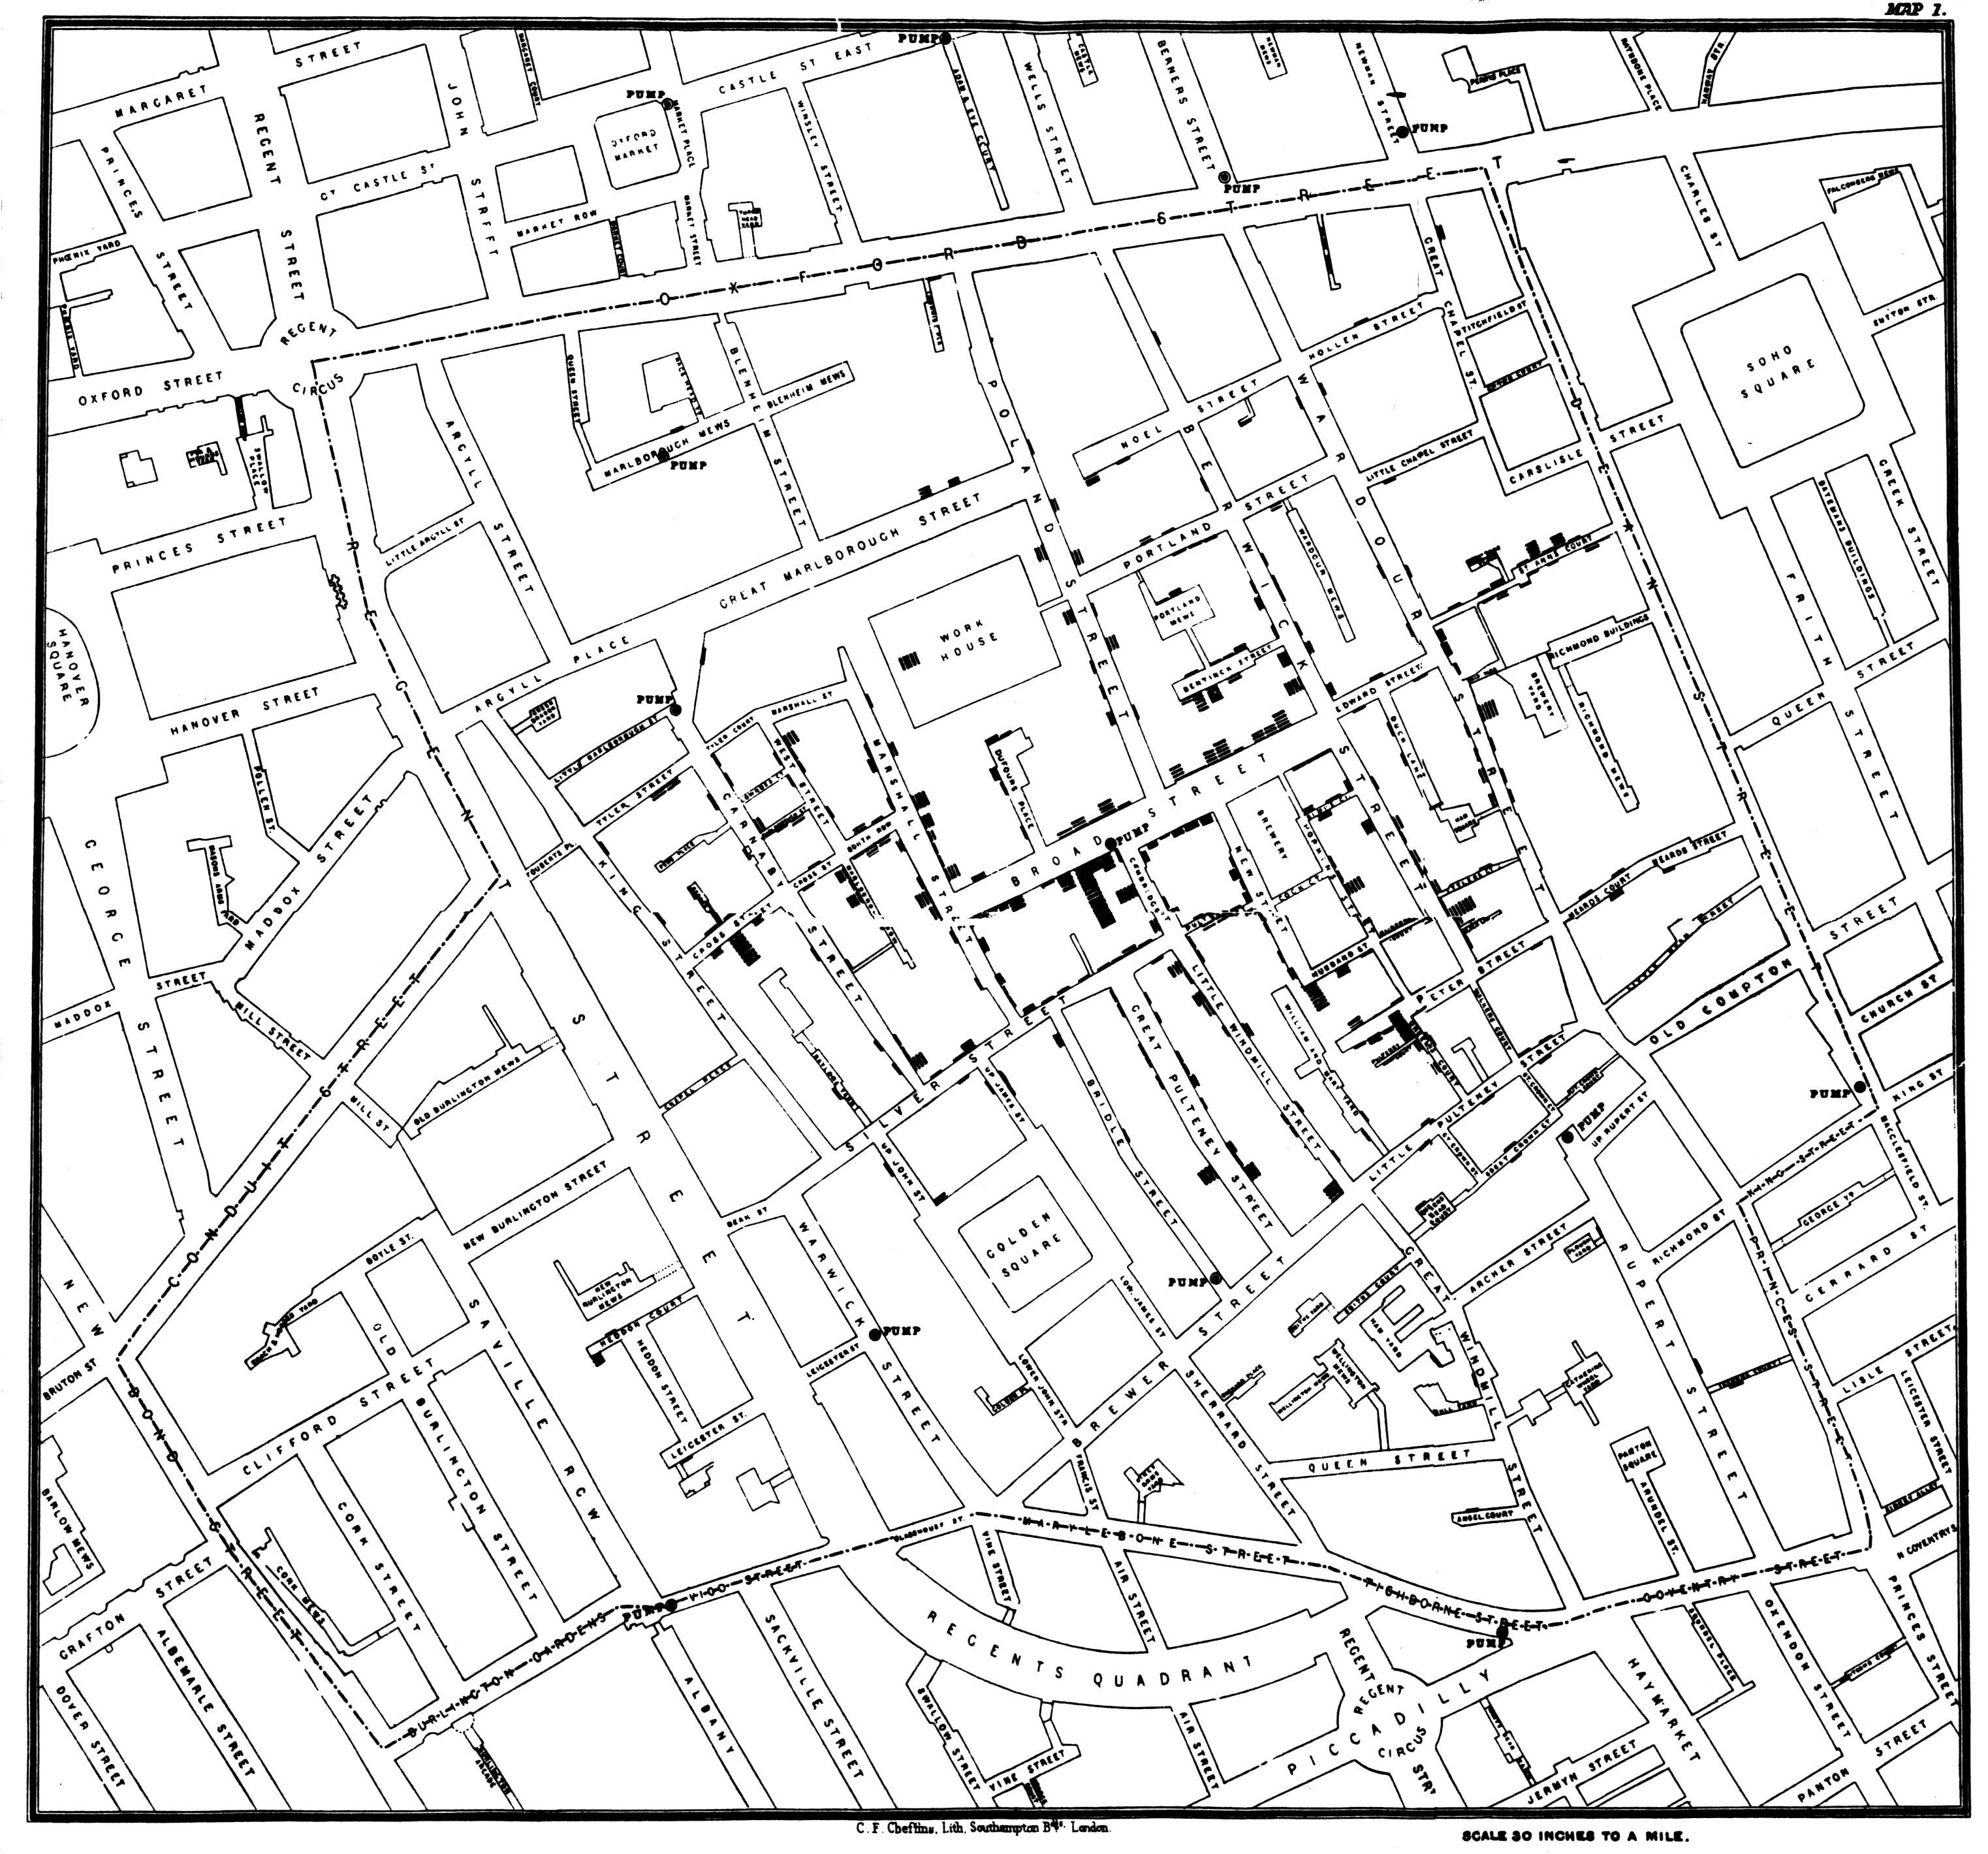
\includegraphics[height=.98\textheight]{images/broadstreet}
\end{center}

{\footnotesize Image source: Public Domain from \href{https://en.wikipedia.org/wiki/File:Snow-cholera-map-1.jpg}{Wikipedia}}

}

% inductive process: map outbreak of cholera; identify pattern
% new theory: cholera is spread by contaminated water
% hypothesis: removing access to contaminated water reduces cholera infection
% later used as an example of the ``Germ theory of disease'' (most closely associated with Louis Pasteur)



\frame{

\frametitle{Observational Equivalence}

\begin{itemize}\itemsep1em
\item Definition: All hypotheses for two (or more) theories are identical
\item What to do?
	\begin{itemize}
	\item Generate more specific expectations % maybe alternative DVs; more fine grained hypothesis; moderators; etc.
	\item Move outside scope conditions
	\item Settle for lack of explanation
	\end{itemize}
\end{itemize}

}


\begin{frame}

\frametitle{Median Voter Theory of Legislatures}

\begin{center}
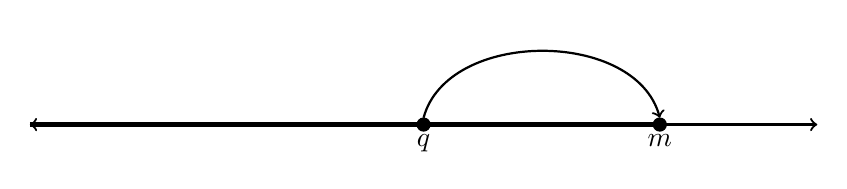
\begin{tikzpicture}
\draw[<->, thick] (-5,2) -- (5,2);
\node<2->[draw,shape=circle,fill=black,scale=0.5] (m) at (3,2) {};
\node<2->[below] at (3,2) {$m$};
\node<3->[draw,shape=circle,fill=black,scale=0.5] (q) at (0,2) {};
\node<3->[below] at (0,2) {$q$};
\draw<4->[->, thick, bend left=75] (q.north) to (m.north);
\draw<5->[ultra thick] (-5,2) to (m);

\end{tikzpicture}
\end{center}

\onslide<5->{If this is true, why do we sometimes see policies left of $m$ in the U.S. House?}

\end{frame}

\begin{frame}

\frametitle{{\large Three Competing Theories}}

\vspace{-2em}

\begin{center}
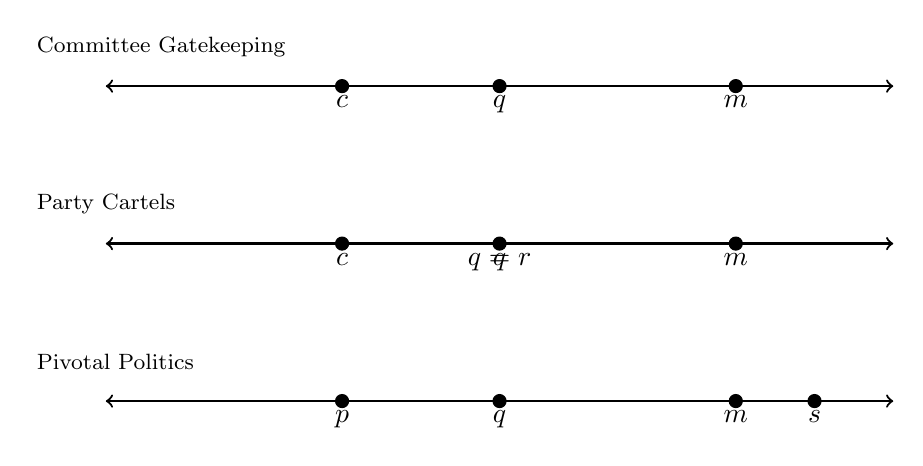
\begin{tikzpicture}
% Committee power
\node[anchor=west] at (-6,2.5) {{\footnotesize Committee Gatekeeping}};
\draw[<->, thick] (-5,2) -- (5,2);
\node<1->[draw,shape=circle,fill=black,scale=0.5] at (3,2) {};
\node<1->[below] at (3,2) {$m$};
\node<1->[draw,shape=circle,fill=black,scale=0.5] at (0,2) {};
\node<1->[below] at (0,2) {$q$};
\node<2->[draw,shape=circle,fill=black,scale=0.5] at (-2,2) {};
\node<2->[below] at (-2,2) {$c$};

% Majority party power
\node[anchor=west] at (-6,0.5) {{\footnotesize Party Cartels}};
\draw[<->, thick] (-5,0) -- (5,0);
\node<1->[draw,shape=circle,fill=black,scale=0.5] at (3,0) {};
\node<1->[below] at (3,0) {$m$};
\node<1->[draw,shape=circle,fill=black,scale=0.5] at (0,0) {};
\node<1-2>[below] at (0,0) {$q$};
\node<3->[below] at (0,0) {$q=r$};
\node<3->[draw,shape=circle,fill=black,scale=0.5] at (-2,0) {};
\node<3->[below] at (-2,0) {$c$};

% Pivotal Politics
\node[anchor=west] at (-6,-1.5) {{\footnotesize Pivotal Politics}};
\draw[<->, thick] (-5,-2) -- (5,-2);
\node<1->[draw,shape=circle,fill=black,scale=0.5] at (3,-2) {};
\node<1->[below] at (3,-2) {$m$};
\node<1->[draw,shape=circle,fill=black,scale=0.5] at (0,-2) {};
\node<1->[below] at (0,-2) {$q$};
\node<4->[draw,shape=circle,fill=black,scale=0.5] at (-2,-2) {};
\node<4->[below] at (-2,-2) {$p$};
\node<4->[draw,shape=circle,fill=black,scale=0.5] at (4,-2) {};
\node<4->[below] at (4,-2) {$s$};


\end{tikzpicture}
\end{center}

{\tiny Adapted From: Krehbiel, Keith. 1999. ``Paradoxes of Parties in Congress.'' \textit{Legislative Studies Quarterly} 24(1): 31--64.\par}

\end{frame}

% how would we resolve these different theories?


\section{Hypothesis Testing}
\frame{\tableofcontents[currentsection]}


\frame{

\frametitle{Hypothesis Testing}

\begin{itemize}\itemsep1em
\item Multiple schools of thought
\item History is conflictual and murky
\item Two strands of literature
	\begin{itemize}
	\item Philosophy of science  % not going to talk about this
	\item Statistics % focus on this perspective, which we'll elaborate mathematically in LT
	\end{itemize}

\end{itemize}

}

% what does it mean to "test" a hypothesis?

\frame{
\frametitle{{\large Principle of Hypothesis Testing}}

\begin{enumerate}\itemsep0.5em
\item Identify and collect data
\item<2-> Data should include:
	\begin{itemize}
	\item Independent variable(s)
	\item Dependent variable(s)
	\end{itemize}
\item<3-> Need variation on both % because we want to observe counterfactuals
\item<4-> Test difference between outcomes when (possibly) causal variable differs
\end{enumerate}

}

\frame{

\frametitle{{\large Forms of Hypothesis Testing}}

\footnotesize

\begin{columns}[T] % align columns
\begin{column}{.4\textwidth}
\begin{block}{Null hypothesis}
Begin with \textit{null hypothesis}\\

\vspace{1em}

Your hypothesis expects an alternative state of the world\\

\vspace{2em}

c/o Ronald Fisher
\end{block}
\end{column}

\begin{column}{.4\textwidth}
\begin{block}{Alternative hypotheses}
Begin with 2(+) alternative hypotheses\\

\vspace{1em}

Accept hypothesis consistent with observation

\vspace{1em}

c/o Jerzy Neyman and Egon Pearson
\end{block}
\end{column}
\end{columns}

}

% today we want to discuss principles of hypothesis testing as a way of thinking independent of statistics

% You've probably previously been exposed to some blend of these ideas



\frame{

\frametitle{Fearon's Counterfactuals}

\begin{itemize}\itemsep0.5em
\item Sometimes we cannot test our hypothesis with actual observations % reasons for this: confounding, no counterfactual case, multiple causality
\item What does Fearon suggest we do?
\end{itemize}


}

% thinking counterfactually
	% can we observe the counterfactual (in another case, in the same case at another time, in a collection of other cases)?
	% if not, can we think about what that counterfactual might look like? 
	% see Fearon's use of ``counterfactual method''; thought experiments; hypothetical reasoning



\frame{

\frametitle{A Good Test}

\small

\begin{itemize}\itemsep-0.1em
\item Correct level of analysis
\item Within scope conditions of theory
\item Well-defined concepts
\item Measures of high construct validity, accuracy, and precision
\item Possible to observe any correlation between potential cause and outcome
\item Consistent with or an improvement upon past methods
\item Test using different data than data used to generate theory % distinguish between training set and test set
\end{itemize}

}


\frame{

\frametitle{Some Testing Challenges}

\begin{enumerate}\itemsep0.5em
\item Deterministic and probabilistic causality
\item Effect heterogeneity
\item Multiple causation
\item Equifinality
\item Confirmation or disconfirmation bias
\end{enumerate}

}





\section{Preview}
\frame{\tableofcontents[currentsection]}


% multiple specific forms of testing, which we'll be exposed to over the coming weeks
	% case studies and comparisons
	% process tracing
	% tabular and visual comparisons
	% regression
	% experimentation

% realizing that we will always be inductive and we may go into the field to test a theory and end up instead generating a new theory



\frame{

\frametitle{Preview of Next Week}

\begin{itemize}\itemsep1em
\item What is a case?
\item What are case studies?
\item How do we use case studies to test and/or build theories?
\end{itemize}

}



\appendix
\frame{}

\end{document}
